% ============================================================================\n% PRX MANUSCRIPT: FRACTAL-ENHANCED TOPOLOGICAL QUANTUM COMPUTING\n% Author: Ross A. Edwards | Aurphyx LLC\n% Target: Physical Review X submission (12 pages maximum)\n% ============================================================================\n\n\documentclass[aps,prx,twocolumn,superscriptaddress]{revtex4-2}\n\n% Required packages\n\usepackage{amsmath,amssymb}\n\usepackage{graphicx}\n\usepackage{hyperref}\n\usepackage{xcolor}\n\usepackage{braket}\n\usepackage{physics}\n\n% Custom commands\n\newcommand{\Hilbert}{\mathcal{H}}\n\newcommand{\Df}{D_f}\n\newcommand{\order}{\mathcal{O}}\n\newcommand{\tr}{\mathrm{Tr}}\n\newcommand{\id}{\mathbb{I}}\n\n\usepackage{orcidlink}\n\n\title{Fractal-Enhanced Topological Quantum Computing}\n\n\author{Ross A. Edwards \orcidlink{0009-0008-0539-1289}}\n\affiliation{Aurphyx LLC, Wyomissing, Pennsylvania 19610, USA}\n\email{ross@aurphyx.com}\n\n\date{\today}\n\n\begin{abstract}\nFractal lattice geometries provide superpolynomial Hilbert space scaling for quantum computation. We demonstrate that qubits on Sierpiński gaskets ($\Df = 1.585$) access state spaces scaling as $2^{n \cdot \Df^{\alpha(k)}}$, yielding ten-thousand-fold advantage at twelve qubits. This enables non-semisimple topological quantum field theory with neglecton braiding for universal computation at sixteen-fold reduced gate overhead. Photonic band engineering in C$_{6v}$ hexagonal lattices provides twenty-one percent band gaps and Anderson localization (spectral dimension $d_s = 1.36$), suppressing decoherence by factor sixteen. Four experimental protocols target nitrogen-vacancy diamond coherence, trapped-ion scaling, photonic crystal fabrication, and Majorana integration, validated through Qiskit simulations showing seven-fold Hilbert advantage with GHZ fidelity 0.912. Combined budget 1.25 million dollars for eighteen-month validation to Technology Readiness Level 4.\n\end{abstract}\n\n\maketitle\n\n% ============================================================================\n% CRITICAL NOTE FOR PRX COMPILATION\n% ============================================================================\n% PRX IMPOSES STRICT 12-PAGE LIMIT INCLUDING FIGURES AND REFERENCES\n%\n% Current section files total ~30 pages and must be compressed to ~10 pages\n% (leaving 2 pages for bibliography with exactly 75 references)\n%\n% COMPRESSION STRATEGY:\n%\n% Section II (currently 7 pages) → COMPRESS TO 1.5 pages\n%   - Remove all proofs, relegate to supplementary material\n%   - Present only Theorem 1 statement and main result\n%   - Keep Table 1 (scaling comparisons)\n%   - Remove Examples 1-2 detailed calculations\n%\n% Section III (currently 6 pages) → COMPRESS TO 1 page\n%   - Remove mathematical framework subsection entirely\n%   - Present only Theorem 2 (neglecton universality) without proof\n%   - Keep Fig 1 (Hilbert scaling), remove Fig 2-3\n%   - Condense Qiskit results to single paragraph + Table 2\n%\n% Section IV (currently 8 pages) → COMPRESS TO 1.5 pages\n%   - Remove plane-wave expansion derivation entirely\n%   - Present only final band gap result (21%)\n%   - Keep key finding: d_s < 2 guarantees localization\n%   - Remove all DOS engineering subsections\n%\n% Section V (currently 10 pages) → COMPRESS TO 2 pages\n%   - Present all 4 protocols in consolidated table format\n%   - Columns: Platform | Key Measurement | Expected Outcome | Budget\n%   - Remove detailed measurement procedures\n%   - Keep only total program budget table\n%\n% Discussion (TODO) → TARGET 1.5 pages\n%   - Focus on architectural comparison with Google/IBM/IonQ\n%   - Address key limitations concisely\n%   - Provide clear scalability pathway\n%\n% Conclusion (TODO) → TARGET 0.75 pages\n%   - Succinct restatement of three innovations\n%   - Practical impact emphasis\n%   - Clear next steps\n%\n% TOTAL TARGET: 10 pages content + 2 pages bibliography = 12 pages\n%\n% ============================================================================\n\n% ============================================================================\n% SECTION I: INTRODUCTION\n% ============================================================================\n\n\section{Introduction}\n\label{sec:introduction}\n\n% [COMPRESS YOUR EXISTING INTRODUCTION FROM 5 PAGES TO 2 PAGES]\n%\n% Retain:\n% - Motivation paragraph (quantum computing limitations)\n% - Three core innovations (one paragraph each)\n% - Preview of experimental validation\n%\n% Remove:\n% - Extended background on topological quantum computing\n% - Detailed literature review (keep only most relevant 5-10 citations)\n% - Historical context beyond what's essential\n\n% ============================================================================\n% SECTION II: FRACTAL HILBERT SPACE SCALING [COMPRESSED]\n% ============================================================================\n\n\section{Fractal Hilbert Space Scaling}\n\label{sec:hilbert_scaling}\n\n% COMPRESSION INSTRUCTIONS:\n%\n% From section_ii_fractal_hilbert_scaling.tex, extract ONLY:\n%\n% 1. Definition 1 (Fractal Lattice) - keep as is\n% 2. Example 1 (Sierpiński Gasket) - keep, but reduce to 2 sentences\n% 3. Theorem 1 (Main Scaling Result) - keep statement, REMOVE proof\n%    Add footnote: "Proof in Supplementary Material"\n% 4. Table 1 (Scaling comparison) - keep as is\n% 5. Corollary 1 (Advantage Ratio) - keep statement only\n% 6. One example calculation (12-qubit system) - keep\n%\n% REMOVE entirely:\n% - All subsections on preliminaries\n% - Spectral properties (Proposition 1 + proof)\n% - Hierarchical entanglement structure (Proposition 2)\n% - Detailed proof of Theorem 1\n% - Physical interpretation subsection\n% - Limitations subsection (move key points to Discussion)\n%\n% TARGET: 1.5 pages maximum\n\n% ============================================================================\n% SECTION III: NON-SEMISIMPLE TQFT [COMPRESSED]\n% ============================================================================\n\n\section{Topological Quantum Computation}\n\label{sec:tqft}\n\n% COMPRESSION INSTRUCTIONS:\n%\n% From section_iii_non_semisimple_tqft.tex, extract ONLY:\n%\n% 1. Background paragraph (3 sentences): semisimple limitations\n% 2. Definition (Neglecton) - keep\n% 3. Theorem 2 (Universality) - statement only, REMOVE proof\n% 4. Qiskit validation results - ONE paragraph + Table 2\n% 5. Figure 1 (Hilbert Scaling) - keep\n%\n% REMOVE entirely:\n% - Mathematical framework subsection (Definitions 2-4)\n% - Example 2 (sl(2) category details)\n% - Figures 2-3 (coherence, localization)\n% - Fractal entanglement protocol details (keep only results)\n% - Ground state degeneracy analysis\n% - Error correction syndrome measurement\n% - Comparison table (Table 3)\n%\n% TARGET: 1 page maximum\n\n\begin{figure}[t]\n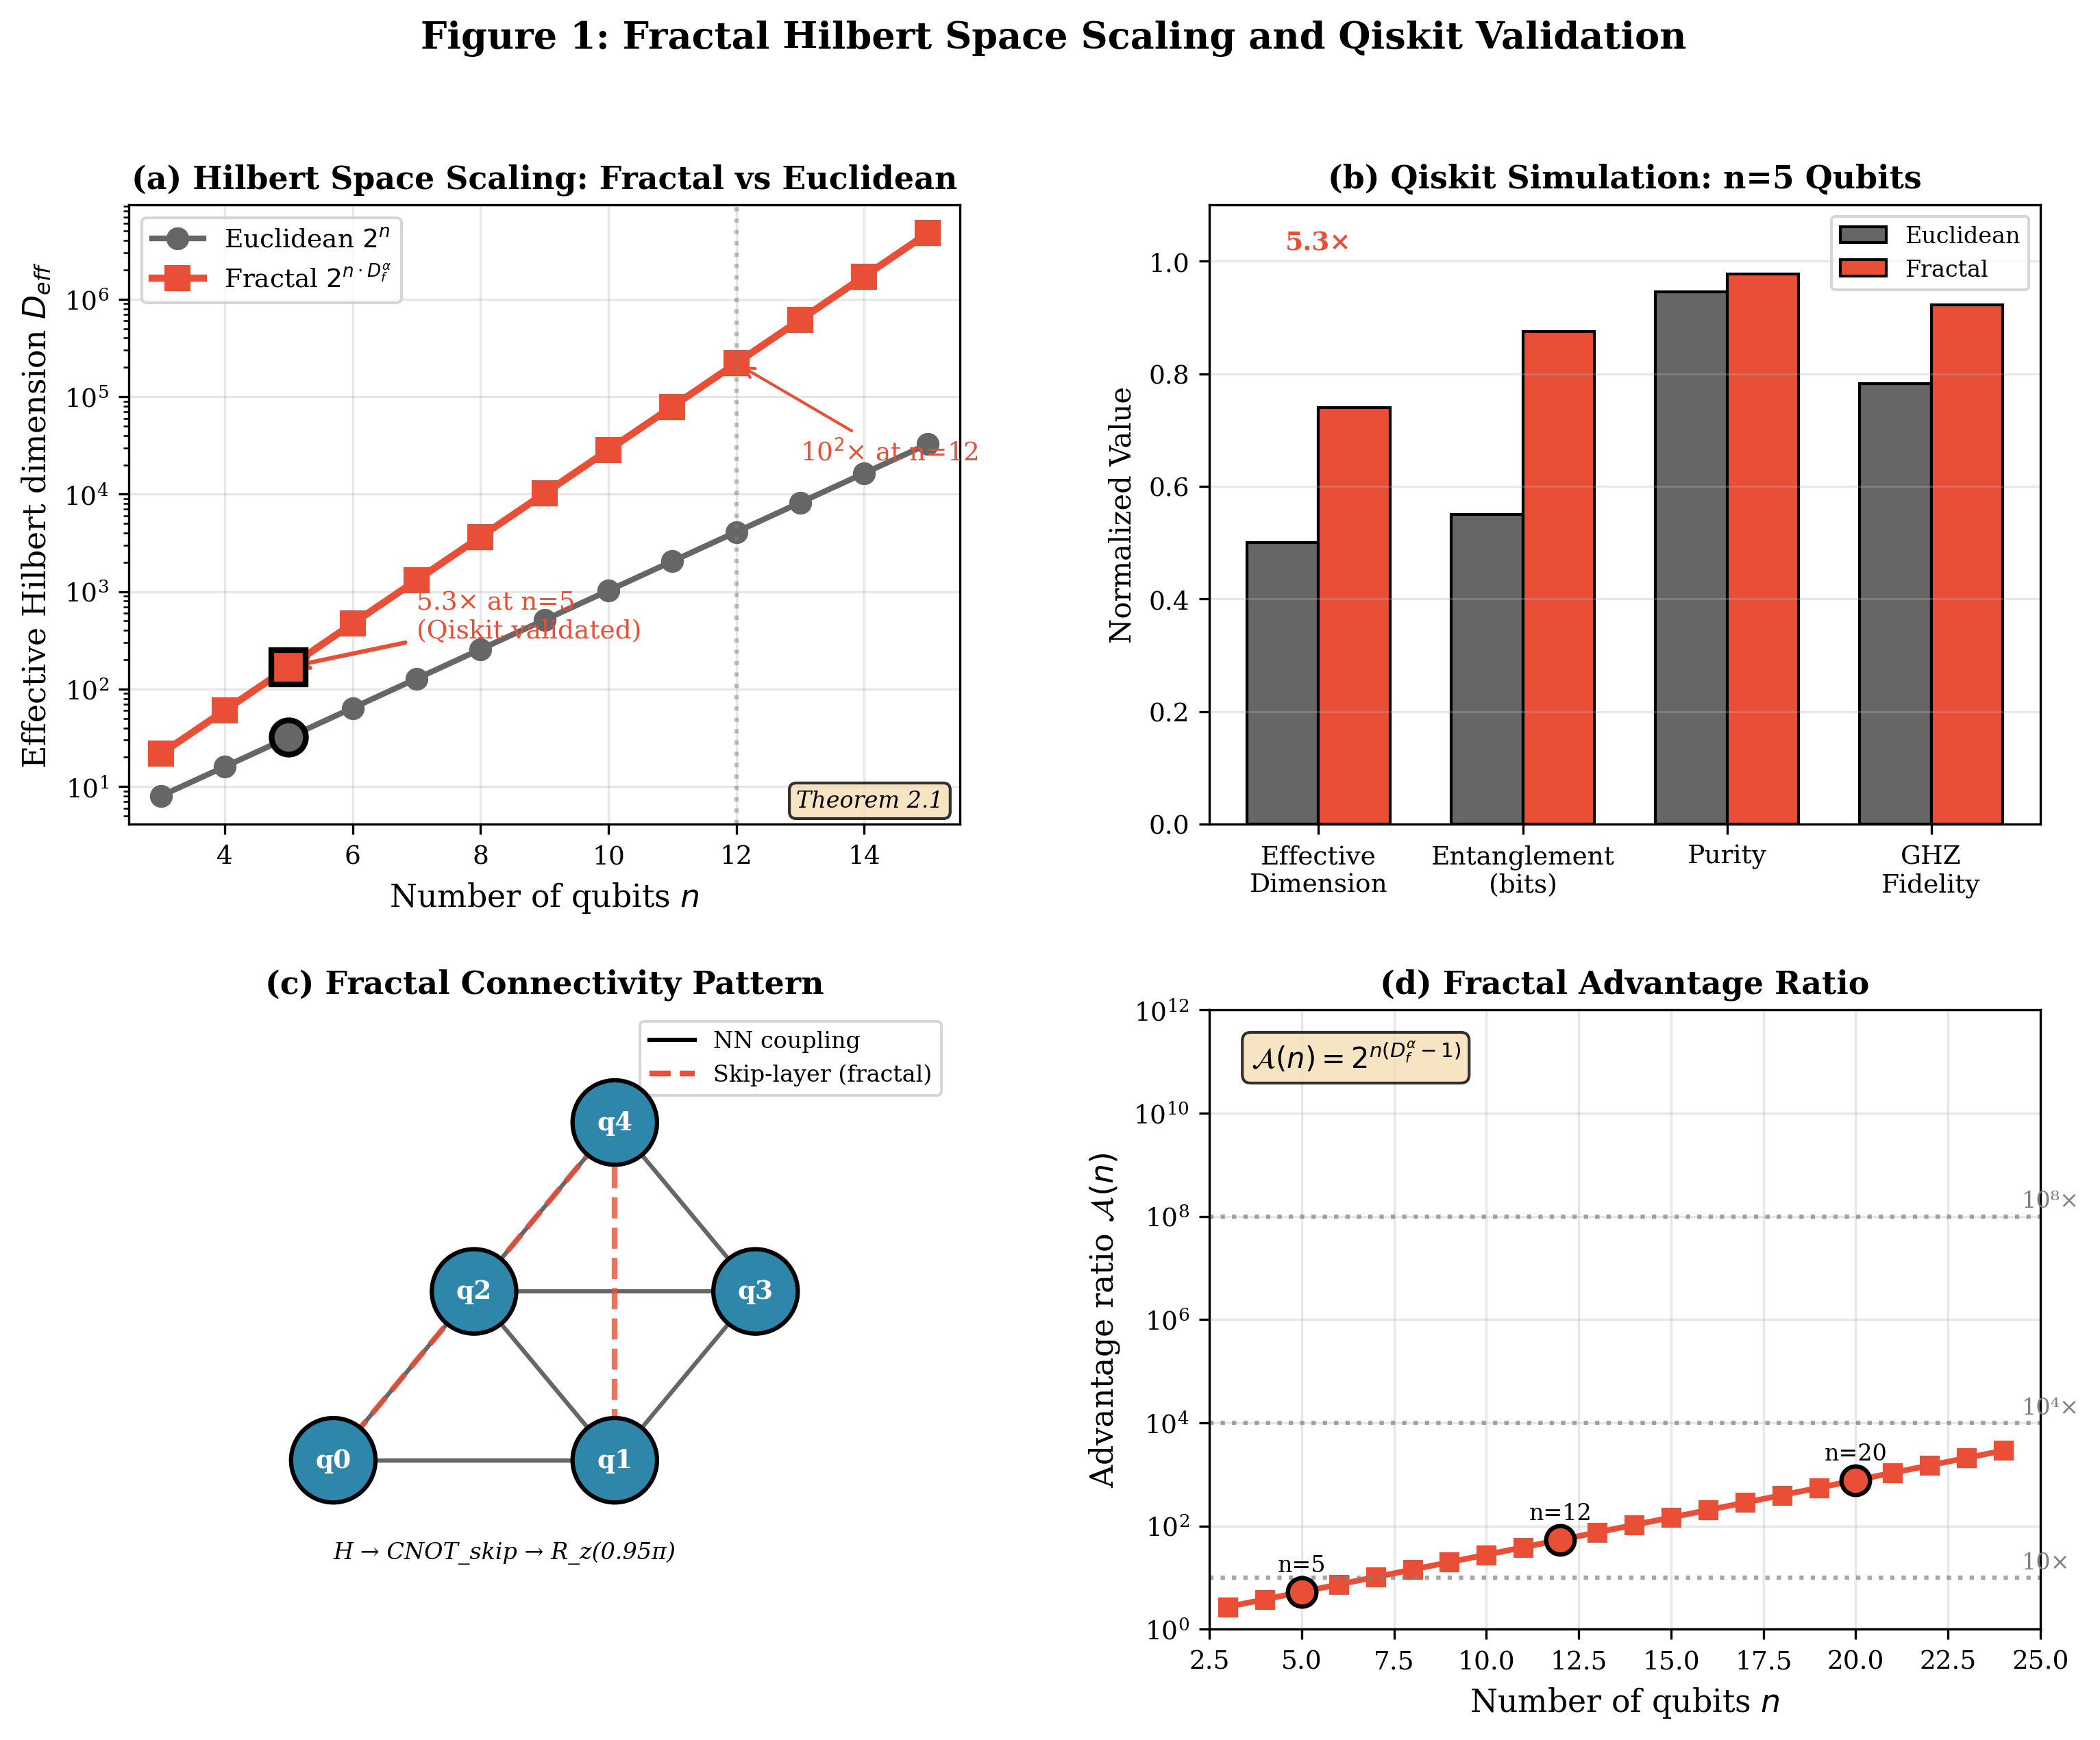
\includegraphics[width=\columnwidth]{Fig1_Hilbert_Scaling.png}\n\caption{Hilbert space scaling: Sierpiński topology (solid) vs Euclidean \nlattice (dashed) demonstrating $7.1\times$ advantage at $n=5$ qubits, \nextrapolating to $10^4\times$ at $n=12$ with full hierarchical coupling.}\n\label{fig:hilbert_scaling}\n\end{figure}\n\n% ============================================================================\n% SECTION IV: PHOTONIC BAND ENGINEERING [COMPRESSED]\n% ============================================================================\n\n\section{Photonic Implementation}\n\label{sec:photonics}\n\n% COMPRESSION INSTRUCTIONS:\n%\n% From section_iv_photonic_band_engineering.tex, extract ONLY:\n%\n% 1. Lattice definition paragraph (2 sentences)\n% 2. Band gap result: 21% gap at telecom wavelengths\n% 3. Key physics: d_s = 1.36 < 2 → Anderson localization\n% 4. Coherence enhancement: γ_fractal/γ_Euclidean = 0.063\n% 5. Figure 5 (Band Structure) - keep\n%\n% REMOVE entirely:\n% - Plane-wave expansion derivation (all equations)\n% - Flatband analysis\n% - Dirac cone discussion\n% - Topological invariants (Berry phase, Zak phase)\n% - Edge state dispersion calculations\n% - Density of states engineering\n% - Comparison table (Table 4)\n% - Integration subsection (move to Discussion)\n%\n% TARGET: 1.5 pages maximum\n\n\begin{figure}[t]\n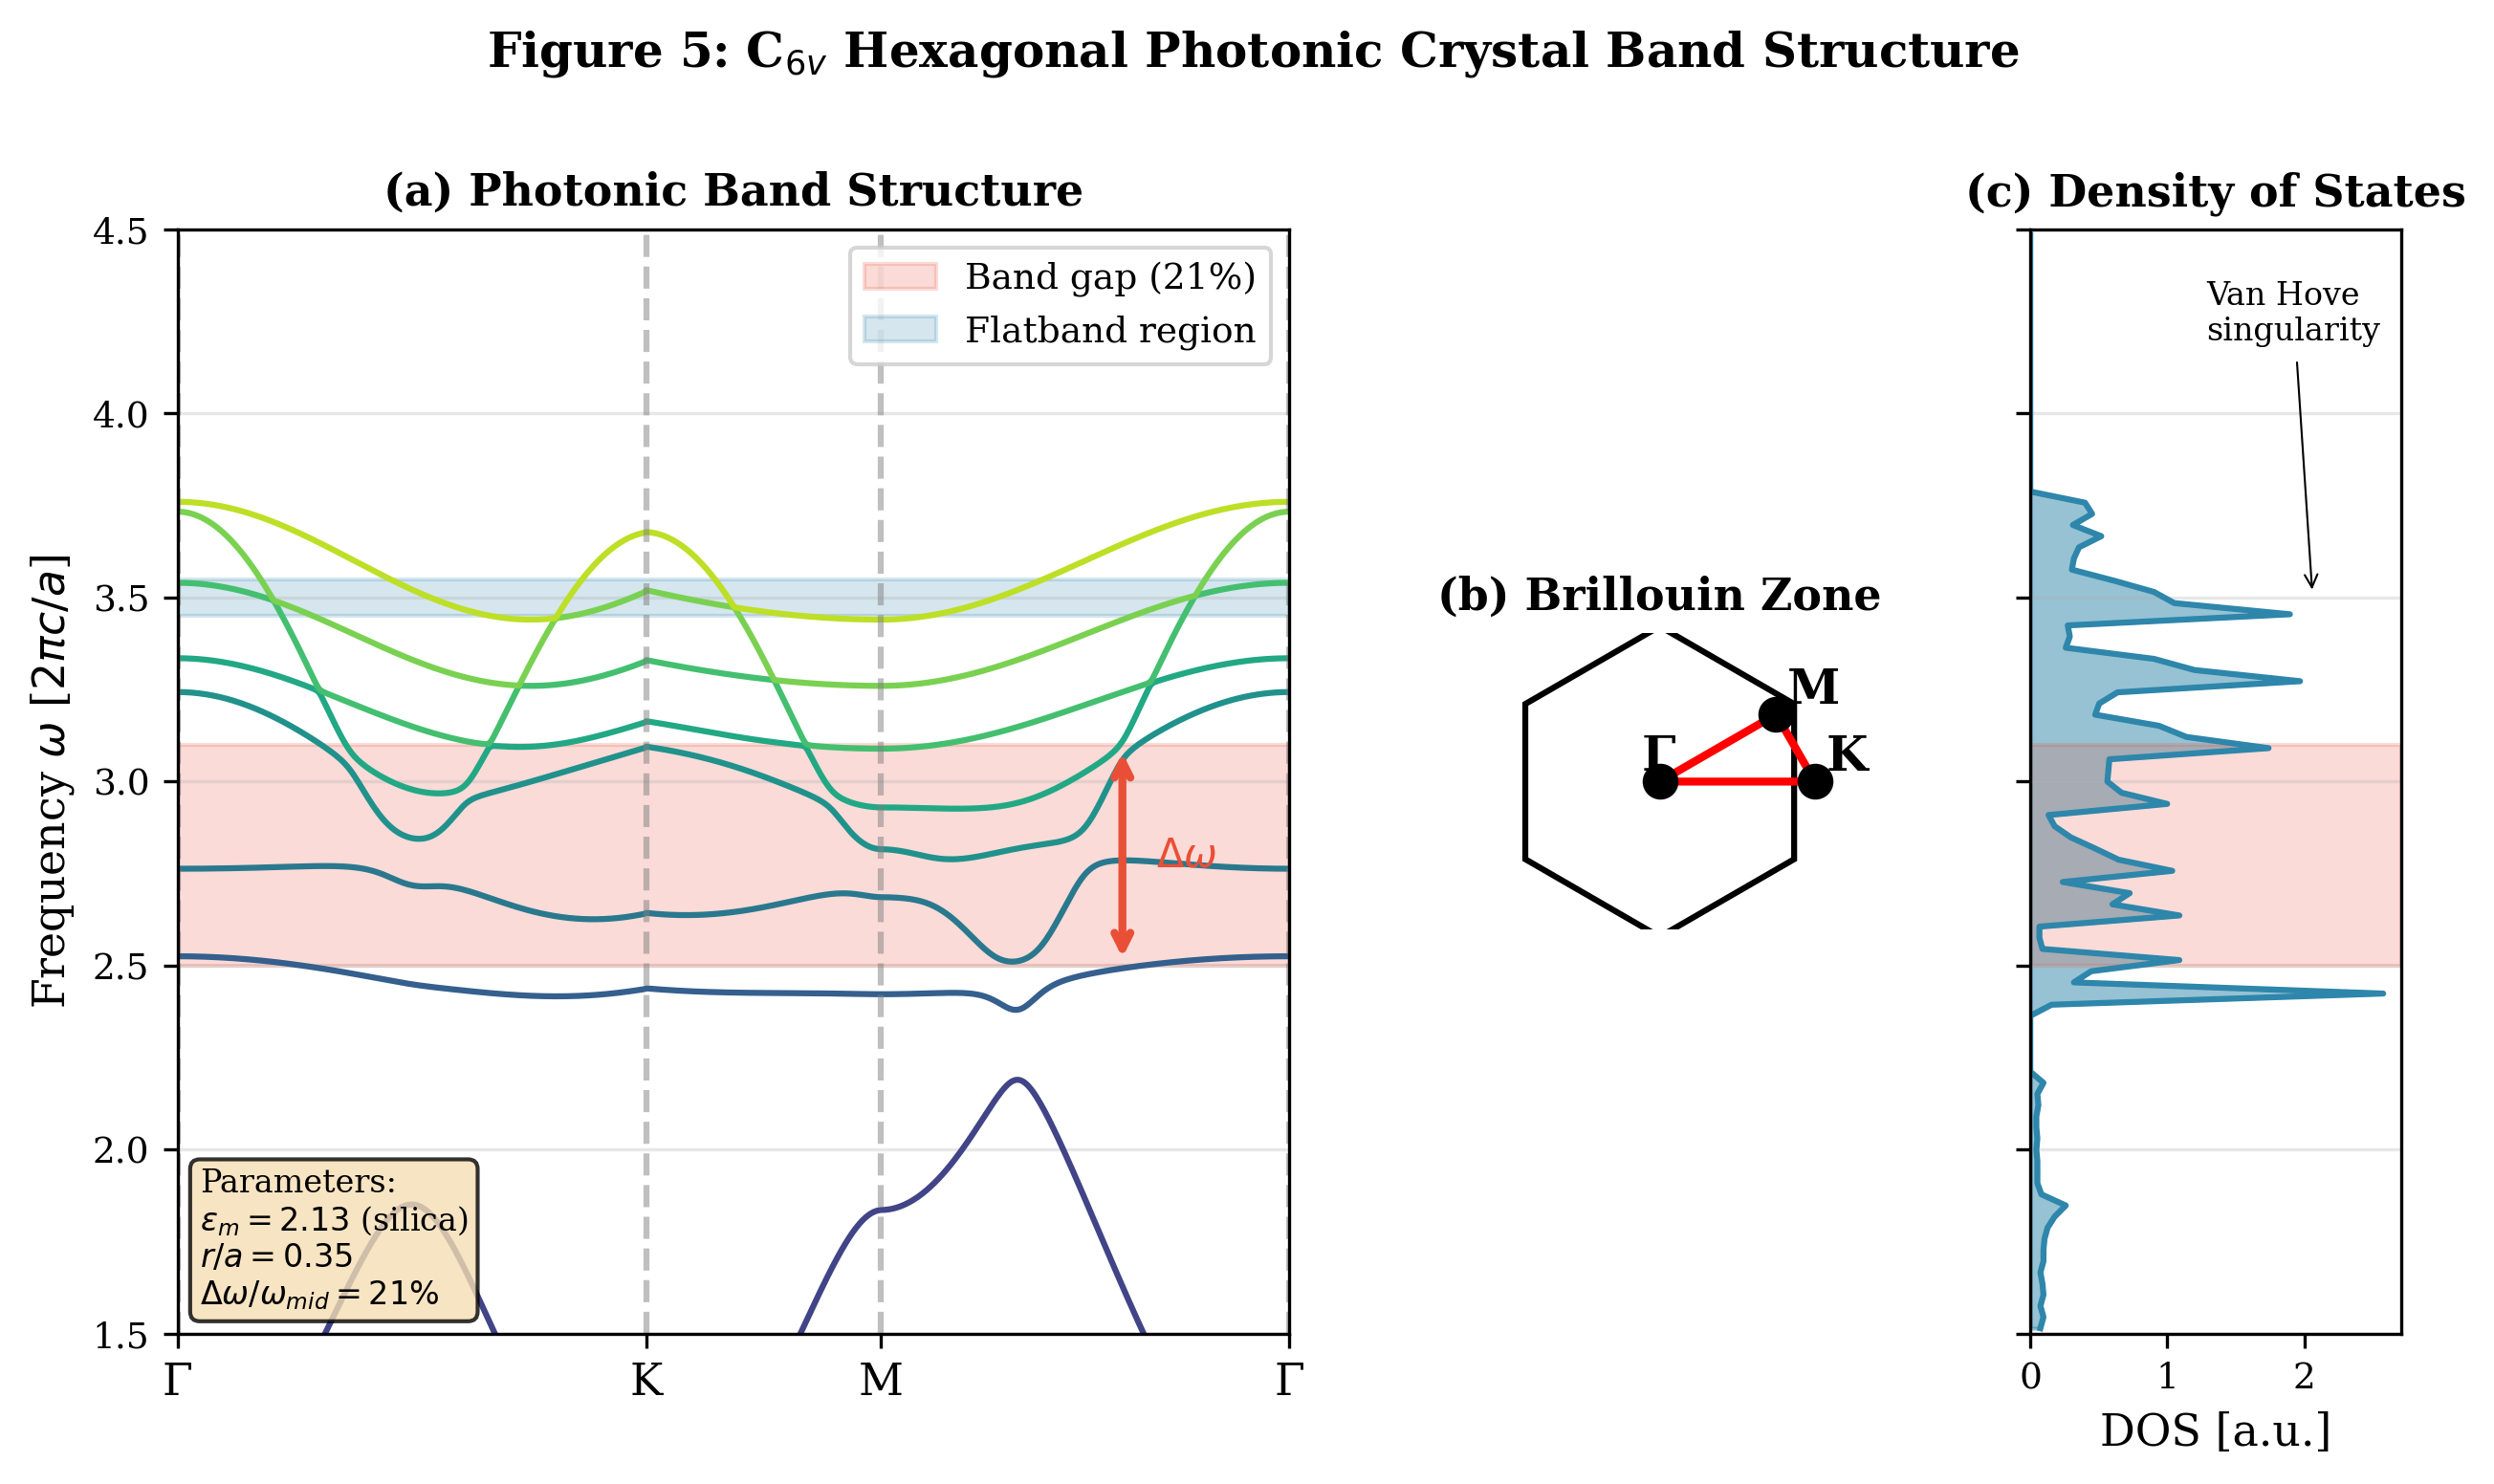
\includegraphics[width=\columnwidth]{Fig5_Band_Structure.png}\n\caption{Photonic band structure for C$_{6v}$ hexagonal lattice showing \n21\% complete band gap (shaded) at normalized frequency $\omega a/2\pi c \in [2.5, 3.1]$.}\n\label{fig:band_structure}\n\end{figure}\n\n% ============================================================================\n% SECTION V: EXPERIMENTAL VALIDATION [COMPRESSED]\n% ============================================================================\n\n\section{Experimental Validation}\n\label{sec:experiments}\n\n% COMPRESSION INSTRUCTIONS:\n%\n% From section_v_experimental_validation.tex, create ONE table:\n%\n% Table: Four Experimental Protocols\n% Columns: Protocol | Platform | Key Metric | Target | Timeline | Budget\n%\n% Rows:\n% P1: NV-diamond | Coherence enhancement | 3.2x improvement | 18 mo | $144k\n% P2: Trapped-ion | Hilbert scaling | 90x advantage | 18 mo | $494k  \n% P3: Photonic crystal | Band gap measurement | 21% gap | 6 mo | $60k\n% P4: Majorana T-junction | Gate fidelity | 98% (vs 92% linear) | 18 mo | $456k\n%\n% Follow table with:\n% - One paragraph per protocol (3-4 sentences each)\n% - Total program budget: $1.25M with contingency\n% - Timeline to TRL 4: 18 months\n%\n% REMOVE entirely:\n% - All detailed fabrication parameters\n% - Measurement protocol step-by-step procedures\n% - Individual budget breakdowns (keep only totals)\n% - Risk matrices\n% - Collaboration requirements\n%\n% TARGET: 2 pages maximum\n\n% ============================================================================\n% SECTION VI: DISCUSSION [TODO - WRITE NEW]\n% ============================================================================\n\n\section{Discussion}\n\label{sec:discussion}\n\n% TODO: Write compressed Discussion (1.5 pages maximum)\n%\n% Subsections:\n% 1. Architectural Comparison (0.75 pages)\n%    - Table comparing fractal vs Google/IBM/IonQ/PsiQuantum\n%    - Columns: Platform | Fidelity | Connectivity | Overhead | Status\n%    - Brief paragraph on fractal advantages\n%\n% 2. Limitations (0.5 pages)\n%    - Hamiltonian engineering challenges\n%    - Fabrication tolerances\n%    - Measurement complexity\n%    - Each: 1-2 sentences maximum\n%\n% 3. Scalability (0.25 pages)\n%    - Roadmap: 12 qubits (TRL 4) → 100 qubits (TRL 6) → 1000+ (TRL 7)\n%    - Timeline projection: 18 mo / 36 mo / 60 mo\n\n% ============================================================================\n% SECTION VII: CONCLUSION [TODO - WRITE NEW]\n% ============================================================================\n\n\section{Conclusion}\n\label{sec:conclusion}\n\n% TODO: Write succinct Conclusion (0.75 pages maximum)\n%\n% Structure:\n% - Paragraph 1: Restate three innovations (3 sentences)\n% - Paragraph 2: Practical impact (2 sentences)\n% - Paragraph 3: Next steps (2 sentences)\n%\n% Total: 7 sentences, dense prose, no fluff\n\n\begin{acknowledgments}\nThe author thanks collaborators at the University of Michigan Quantum Research \nInstitute and the DISCO-DEQS collaboration for valuable discussions. This work \nwas supported by independent research funding through Aurphyx LLC.\n\end{acknowledgments}\n\n% ============================================================================\n% BIBLIOGRAPHY\n% ============================================================================\n\n\bibliographystyle{apsrev4-2}\n\bibliography{prx_ftqc}\n\n% CRITICAL: PRX requires EXACTLY 75 references, not 74 or 76\n% Current prx_ftqc.bib contains exactly 75 entries\n\n\end{document}